\vbox to \myposterheight{%
\begin{block}{Parametric formulation of the adjoint operator of the model}
	\begin{itemize}
		\item Adjoint operator of the linear operator $\mathcal{H} \left\lbrace \vec{\reflectivity} \right\rbrace$ described in~\eqref{eq_inv_problem_cont_domain} is defined as:
		\begin{align}
		\label{eq_continuous_adjoint}
		\mathcal{H}^\dagger \left\lbrace m \right\rbrace \left(\vec{r}^n\right) = \sum \limits_{\vec{p}^i \in \Pi} o_d \left(\vec{r}^n, \vec{p}^i\right) \int \limits_{\tau \in \R} m \left(\vec{p}^i, \tau \right) u\left( t_{Tx} \left(\vec{r}^n\right) + t_{Rx} \left( \vec{r}^n, \vec{p}^i \right) - \tau\right) d\tau
		\end{align}
		where $u\left(t\right) = v_{pe} \left(-t\right)$ is the matched filter of the pulse shape
		\item Discretization of the adjoint operator expressed as:
		\begin{align}
		\label{eq_adjoint_discrete}
		\mathcal{H}_d^\dagger \left\lbrace\vec{m}\right\rbrace \left(\vec{r}^n\right) = \sum \limits_{\vec{p}^i \in \Pi} \omega^n o_d \left(\vec{r}^n, \vec{p}^i\right) \psi \left(t_{Tx}\left(\vec{r}^n\right) + t_{Rx} \left( \vec{r}^n, \vec{p}^i \right) \right) \hat{\vec{m}},
		\end{align}
		where $\hat{\vec{m}} = \vec{m} \ast_t \vec{u}$, $\psi$ is a \num{1}D-interpolation kernel and $\omega^n$ accounts for the integration weight
	\end{itemize}
\end{block}
\vfill
%----------------------------------------------------------------------------------------
%	IMAGE RECONSTRUCTION PROCEDURE
%----------------------------------------------------------------------------------------
\begin{block}{Image reconstruction procedure}
	\begin{itemize}
		\item Linear measurement operator $\mathcal{H}_d \left\lbrace \vec{\reflectivity}\right\rbrace$ defines the following inverse problem:
		\begin{align}
			\vec{m} = \mat{H}_d \vec{\reflectivity} + \vec{\nu}
		\end{align}
		where $\mat{H}_d \in \R^{N_{el}N_t \times N_xN_z}$ matrix associated with the linear measurement model and $\vec{\nu} \in \R^{N_{el}N_t}$ noise due to  model discrepancy and discretization
		\item Sparse regularization to solve the problem
		\begin{align}
			\label{eq_regularization_problem}
			\min \limits_{\vec{\reflectivity} \in \R^{N_xN_z}} \lambda \mathcal{R} \left(\vec{\reflectivity}\right) + \frac{1}{2} \twonorm{\mat{H}_d \vec{\reflectivity} - \vec{m}}^2
		\end{align}
		where $\mathcal{R} \left(\vec{\reflectivity}\right)$ prior term and $\lambda \in \R_+$ regularization parameter
		\item Two priors considered in this study:
		\begin{itemize}
			\item $\ell_p$-norm to the power of $p$: $\mathcal{R}\left(\vec{\reflectivity}\right) = \pnorm{\vec{\reflectivity}}^p$, $p \geq 1$;
			\item $\ell_1$-norm in the SA model: $\mathcal{R}\left(\vec{\reflectivity}\right) = \onenorm{\Psi^\dagger\reflectivity}$, where $\Psi = \frac{1}{\sqrt{q}}\left[\Psi_1,...,\Psi_q\right]$, with $\Psi_i$ the $i$-th Daubechies wavelet.
		\end{itemize}
	\end{itemize}
\end{block}
\vfill
%----------------------------------------------------------------------------------------
%	IMPLEMENTATION OF USSR
%----------------------------------------------------------------------------------------
\begin{block}{Implementation of USSR}
	\begin{itemize}
		\item USSR implemented on GPU platforms and on multi-threaded CPU platforms
		\item \num{200} iterations of the fast iterative shrinkage thresholding algorithm used for reconstruction 
		\item Reconstructions of images from PICMUS dataset~(1 PW insonification) take around \SI{4.5}{\second} on an NVIDIA Titan X GPU card
		\item Code available on GitHub: \url{https://github.com/LTS5/USSR}
	\end{itemize}
\end{block}
%----------------------------------------------------------------------------------------
%	RECONSTRUCTED IMAGES
%----------------------------------------------------------------------------------------
\begin{block}{Reconstructed B-mode images}
	
\newlength{\CohSubFigWidth}
\newlength{\CohSubFigHeight}
\setlength{\CohSubFigWidth}{0.24\columnwidth}
\settoheight{\CohSubFigHeight}{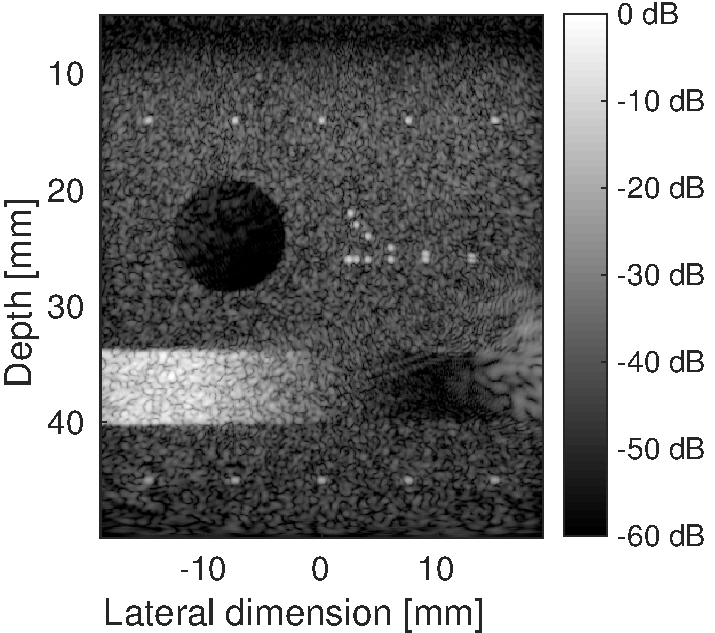
\includegraphics[width=\CohSubFigWidth]{Figures/das_dataset_rf_numerical_transmission_1_nbPW_1.pdf}}
\begin{figure}[htb]
	% Maximum length
	\hfill%
	\subcaptionbox{\label{fig_numerical_DAS}}{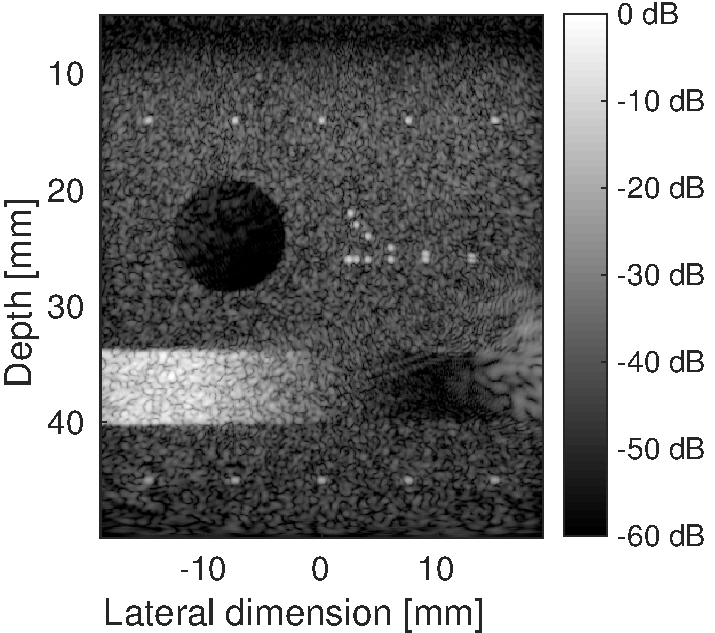
\includegraphics[height=\CohSubFigHeight]{Figures/das_dataset_rf_numerical_transmission_1_nbPW_1.pdf}}\hfill%
	\subcaptionbox{\label{fig_numerical_DAS_5}}{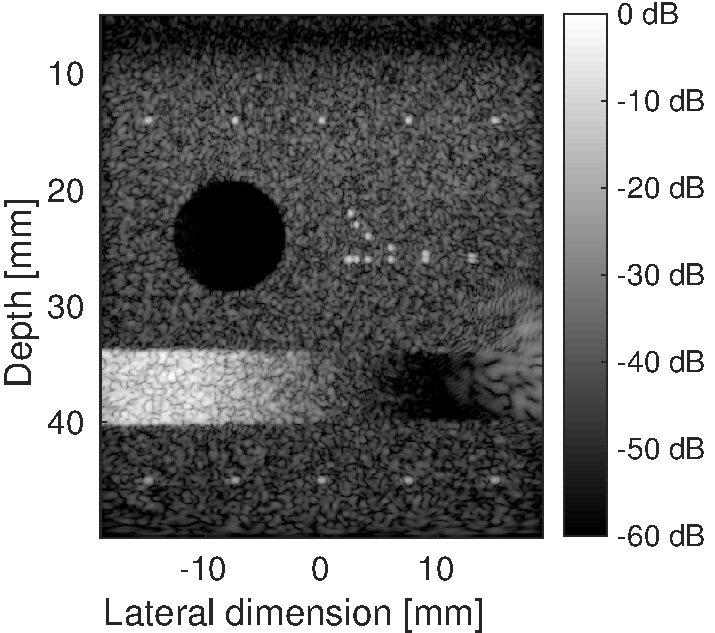
\includegraphics[height=\CohSubFigHeight]{Figures/das_dataset_rf_numerical_transmission_1_nbPW_5.pdf}}\hfill%
	\subcaptionbox{\label{fig_numerical_FISTA}}{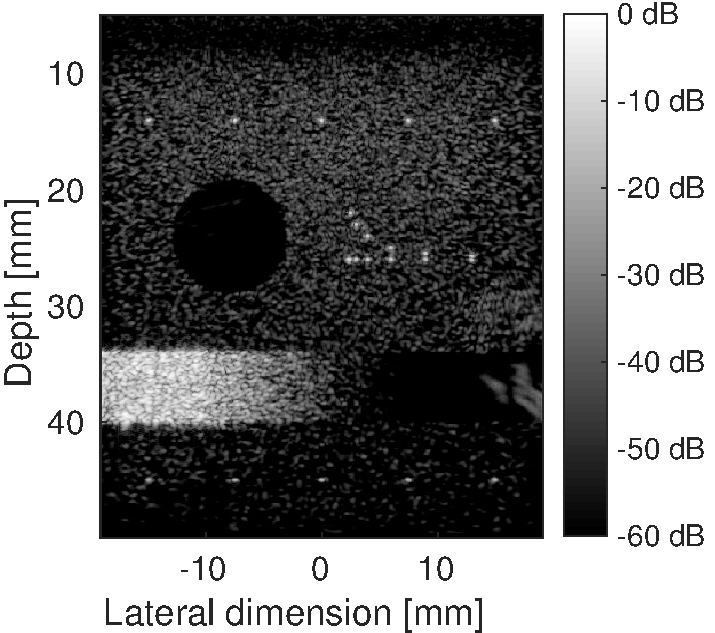
\includegraphics[height=\CohSubFigHeight]{Figures/FISTA_dataset_rf_numerical_transmission_1_nbPW_1.pdf}}\hfill%
	\subcaptionbox{\label{fig_numerical_FISTALP}}{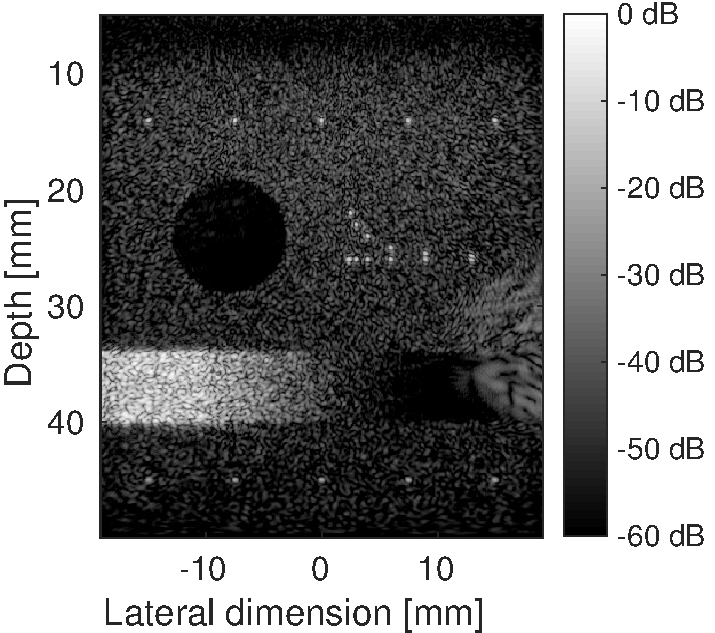
\includegraphics[height=\CohSubFigHeight]{Figures/FISTALP_dataset_rf_numerical_transmission_1_nbPW_1.pdf}}\hfill\null%
	
	\hfill%
	\subcaptionbox{\label{fig_carotid_DAS}}{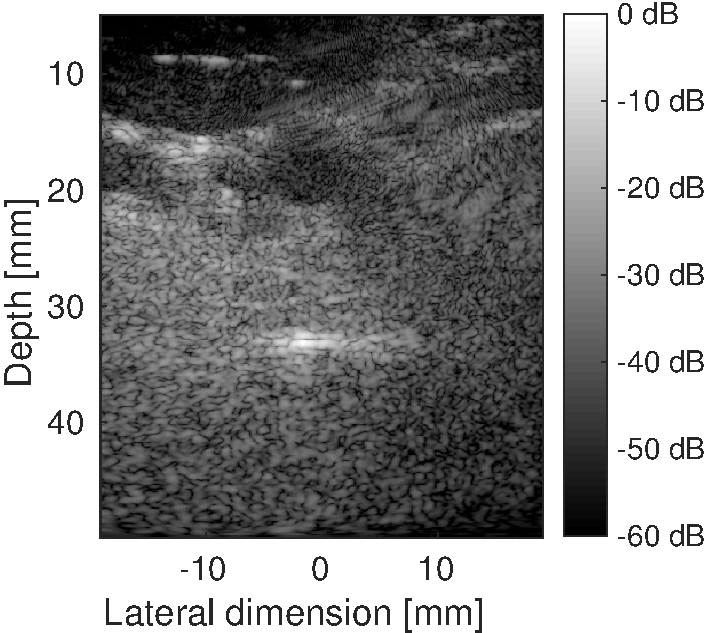
\includegraphics[height=\CohSubFigHeight]{Figures/das_carotid_cross_expe_dataset_rf_nbPW_1.pdf}}\hfill%
	\subcaptionbox{\label{fig_carotid_DAS_5}}{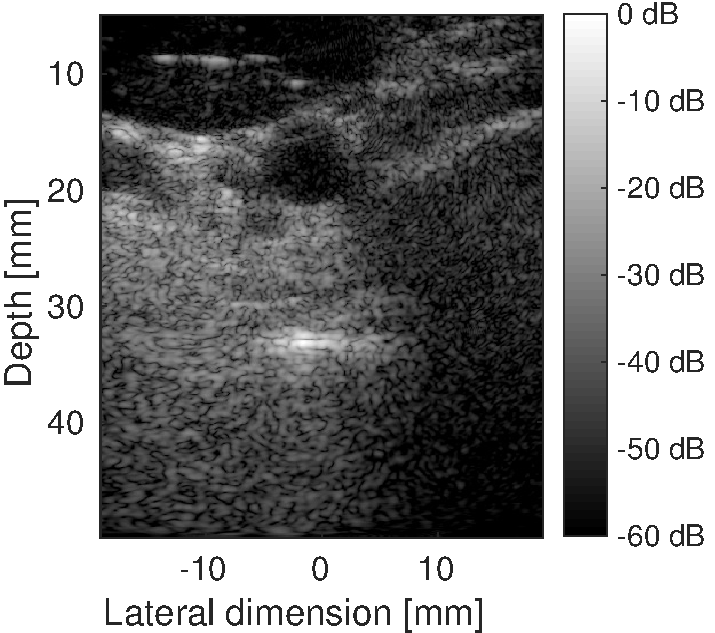
\includegraphics[height=\CohSubFigHeight]{Figures/das_carotid_cross_expe_dataset_rf_nbPW_5.pdf}}\hfill%
	\subcaptionbox{\label{fig_carotid_FISTA}}{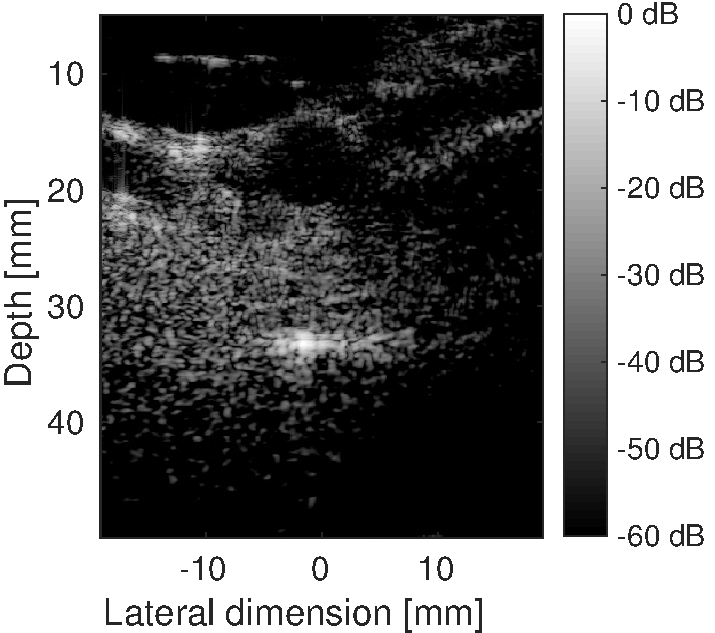
\includegraphics[height=\CohSubFigHeight]{Figures/FISTA_carotid_cross_expe_dataset_rf.pdf}}\hfill%
	\subcaptionbox{\label{fig_carotid_FISTALP}}{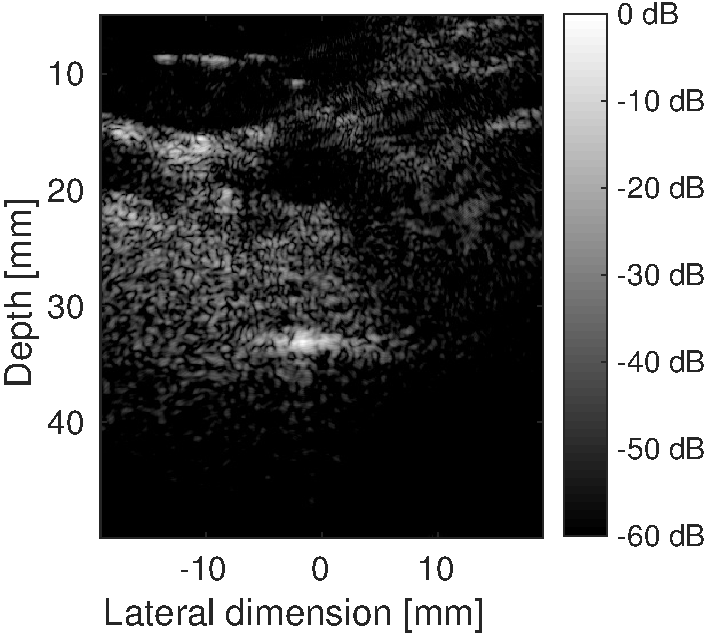
\includegraphics[height=\CohSubFigHeight]{Figures/FISTALP_carotid_cross_expe_dataset_rf.pdf}}\hfill\null%
	\caption{Image of the numerical phantom of PICMUS dataset reconstructed with (a) DAS - 1 PW insonification, (b) DAS - 5 PW insonifications, (c) USSR-SA - 1 PW insonification, (c) USSR - $\ell_p$ - 1 PW insonification; Image of the \textit{in-vivo} carotid reconstructed with (e) DAS - 1 PW insonification, (f) DAS - 5 PW insonifications, (g) USSR-SA - 1 PW insonification, (h) USSR-$\ell_p$ - 1 PW insonification.}
	\label{fig_Bmode}
\end{figure}
	
\end{block}
\vfill

%----------------------------------------------------------------------------------------
%	CONCLUSION
%----------------------------------------------------------------------------------------
\begin{block}{Conclusion and perspectives}
	\begin{enumerate}
		\item We propose USSR: an UltraSound Sparse Regularization framework
		\begin{itemize}
			\item Matrix-free and highly parallelizable formulations of measurement model and adjoint
			\item Two priors: $\ell_p$-norm in the image domain and $\ell_1$-norm in a sparsity averaging model
		\end{itemize}
		\item The proposed approach leads to high-quality at fast rates, with low-memory footprint
		\item Current work focuses on optimizing the code
	\end{enumerate}
\end{block}
\vfill
%----------------------------------------------------------------------------------------
%	BIBLIOGRAPHY
%----------------------------------------------------------------------------------------
%\begin{block}{References}
%	\printbibliography
%\end{block}
%\vfill
%----------------------------------------------------------------------------------------
%	ACKNOWLEDGMENTS
%----------------------------------------------------------------------------------------
\begin{block}{Acknowledgments}
	This work was supported in part by the UltrasoundToGo RTD project (no. 20NA21 145911), evaluated by the Swiss NSF and funded by Nano-Tera.ch with Swiss Confederation financing.
\end{block}
}%